%\section{Systematics Uncertainties on the Background Prediction}
%\label{sec:systematics}

\subsection{Uncertainty on the \ttll\ Acceptance}

The \ttbar\ background prediction is obtained from MC, with corrections
derived from control samples in data. The uncertainty associated with
the theoretical modeling of the \ttbar\ production and decay is
estimated by comparing the background predictions obtained using 
alternative MC samples. It should be noted that the full analysis is
performed with the alternative samples under consideration, 
including the derivation of the various data-to-MC scale factors. 
The variations considered are

\begin{itemize}
\item Top mass: The alternative values for the top mass differ
  from the central value by $5~\GeV$: $m_{\mathrm{top}} = 178.5~\GeV$ and $m_{\mathrm{top}}
  = 166.5~\GeV$.
\item Jet-parton matching scale: This corresponds to variations in the
  scale at which the Matrix Element partons from Madgraph are matched
  to Parton Shower partons from Pythia. The nominal value is
  $x_q>20~\GeV$. The alternative values used are $x_q>10~\GeV$ and
  $x_q>40~\GeV$.
\item Renormalization and factorization scale: The alternative samples
  correspond to variations in the scale $\times 2$ and $\times 0.5$. The nominal
  value for the scale used is $Q^2 = m_{\mathrm{top}}^2 +
  \sum_{\mathrm{jets}} \pt^2$.
\item Alternative generators: Samples produced with different
  generators include MC@NLO and Powheg (NLO generators) and
  Pythia (LO). It may also be noted that MC@NLO uses Herwig6 for the 
  hadronisation, while POWHEG uses Pythia6.
\item Modeling of taus: The alternative sample does not include
  Tauola and is otherwise identical to the Powheg sample. 
\item The PDF uncertainty is estimated following the PDF4LHC
  recommendations[CITE]. The events are reweighted using alternative
  PDF sets for CT10 and MSTW2008 and the uncertainties for each are derived using the
  alternative eigenvector variations and the ``master equation''. In
  addition, the NNPDF2.1 set with 100 replicas. The central value is
  determined from the mean and the uncertainty is derived from the
  $1\sigma$ range. The overall uncertainty is derived from the envelope of the
  alternative predictions and their uncertainties. 
\end{itemize}


\begin{figure}[hbt]
  \begin{center}
	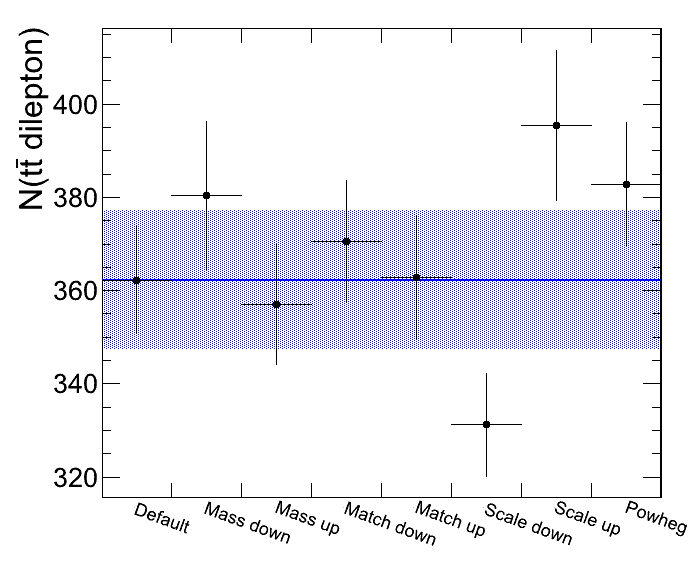
\includegraphics[width=0.8\linewidth]{plots/n_dl_syst_comp.png}
	\caption{
	  \label{fig:ttllsyst}%\protect 
          Central Prediction
          Band: 
          - total stat. error for all Data and MC samples
          - N jets scaling uncertainty (ISR/FSR)
          Alternative Sample Predictions
          Error bars: uncorrelated stat. error from alternative ttbar sample only}
      \end{center}
    \end{figure}



%
%
%The methodology for determining the systematics on the background
%predictions has not changed with respect to the nominal analysis.
%Because the template method has not changed, the same 
%systematic uncertainty is assessed on this prediction (32\%).
%The 50\% uncertainty on the WZ and ZZ background is also unchanged.
%The systematic uncertainty in the OF background prediction based on 
%e$\mu$ events has changed, due to the different composition of this
%sample after vetoing events containing b-tagged jets.
%
%As in the nominal analysis, we do not require the e$\mu$ events
%to satisfy the dilepton mass requirement and apply a scaling factor K,
%extracted from MC, to account for the fraction of e$\mu$ events
%which satisfy the dilepton mass requirement. This procedure is used
%in order to improve the statistical precision of the OF background estimate.
%
%For the selection used in the nominal analysis, 
%the e$\mu$ sample is completely dominated by $t\bar{t}$
%events, and we observe that K is statistically consistent with constant with
%respect to the \MET\ requirement. However, in this analysis, the $t\bar{t}$
%background is strongly suppressed by the b-veto, and hence the non-$t\bar{t}$
%backgrounds (specifically, $Z\to\tau\tau$ and VV) become more relevant. 
%At low \MET, the $Z\to\tau\tau$ background is pronounced, while $t\bar{t}$
%and VV dominate at high \MET\ (see App.~\ref{app:kinemu}).
%Therefore, the sample composition changes
%as the \MET\ requirement is varied, and as a result K depends
%on the \MET\ requirement. 
%
%We thus measure K in MC separately for each
%\MET\ requirement, as displayed in Fig.~\ref{fig:kvmet} (left).
%%The systematic uncertainty on K is determined separately for each \MET\
%%requirement by comparing the relative difference in K in data vs. MC.
%The values of K used are the MC predictions 
%%and the total systematic uncertainty on the OF prediction 
%%as shown in 
%(Table \ref{fig:kvmettable}).
%The contribution to the total OF prediction systematic uncertainty 
%from K is assessed from the ratio of K in data and MC,
%shown in Fig.~\ref{fig:kvmet} (right).
%The ratio is consistent with unity to roughly 17\%, 
%so we take this value as the systematic from K.
%17\% added in quadrature with 7\% from 
%the electron to muon efficieny ratio 
%(as assessed in the inclusive analysis)
%yields a total systematic of $\sim$18\% 
%which we round up to 20\%.
%For \MET\ $>$ 150, there are no OF events in data inside the Z mass window
%so we take a systematic based on the statistical uncertainty
%of the MC prediction for K. 
%This value is 25\% for \MET\ $>$ 150 GeV and 60\% for \MET\ $>$ 200 GeV.
%%Although we cannot check the value of K in data for \MET\ $>$ 150
%%because we find no OF events inside the Z mass window for this \MET\ 
%%cut, the overall OF yields with no dilepton mass requirement 
%%agree to roughly 20\% (9 data vs 7.0 $\pm$ 1.1 MC).
%
%
%%Below Old
%
%%In reevaluating the systematics on the OF prediction, however,
%%we observed a different behavior of K as a function of \MET\ 
%%as was seen in the inclusive analysis. 
%
%%Recall that K is the ratio of the number of \emu\ events
%%inside the Z window to the total number of \emu\ events.
%%In the inclusive analysis, it is taken from \ttbar\ MC
%%and used to scale the inclusive \emu\ yield in data.
%%The yield scaled by K is then corrected for 
%%the $e$ vs $\mu$ efficiency difference to obtain the 
%%final OF prediction.
%
%%Based on the plot in figure \ref{fig:kvmet}, 
%%we choose to use a different
%%K for each \MET\ cut and assess a systematic uncertainty
%%on the OF prediction based on the difference between 
%%K in data and MC. 
%%The variation of K as a function of \MET\ is caused 
%%by a change in sample composition with increasing \MET.
%%At \MET\ $<$ 60 GeV, the contribution of Z plus jets is
%%not negligible (as it was in the inclusive analysis)
%%because of the b veto. (See appendix \ref{app:kinemu}.)
%%At higher \MET, \ttbar\ and diboson backgrounds dominate.
%
%
%
%
%\begin{figure}[hbt]
%  \begin{center}
%	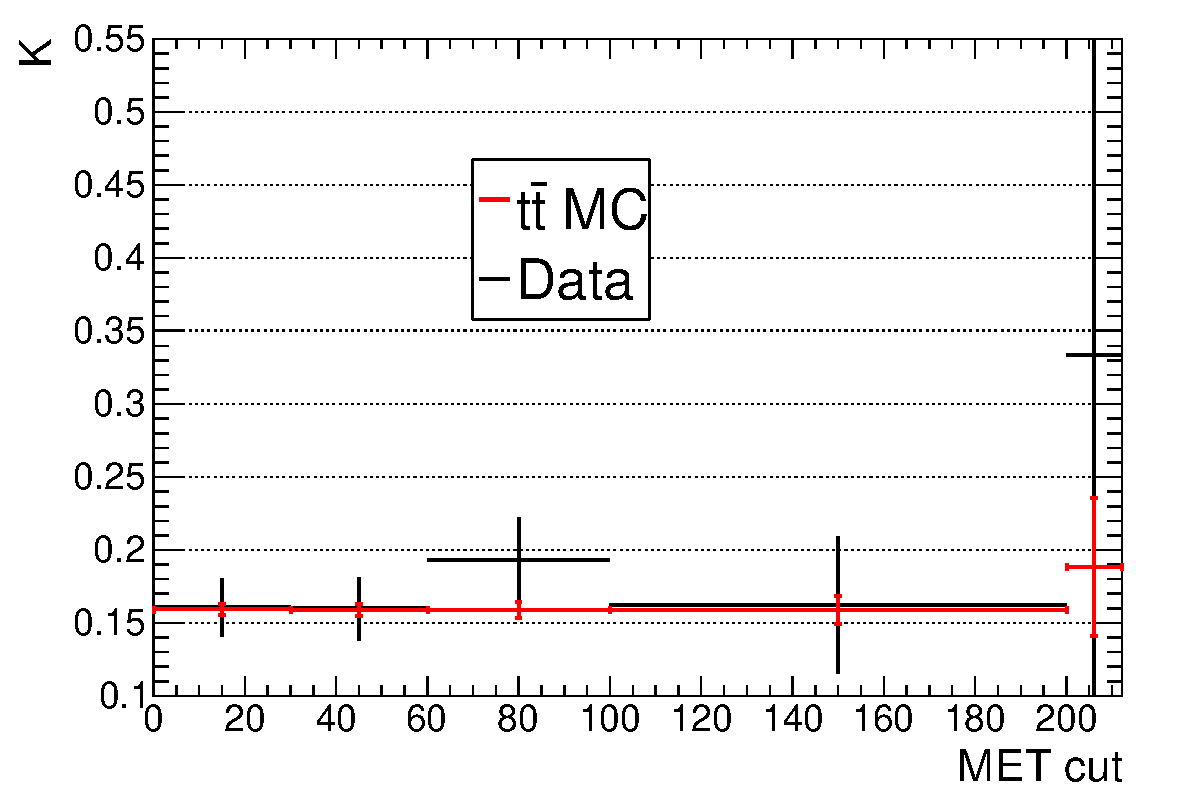
\includegraphics[width=0.48\linewidth]{plots/kvmet_data_ttbm.pdf}
%	\includegraphics[width=0.48\linewidth]{plots/kvmet_ratio.pdf}
%	\caption{
%	  \label{fig:kvmet}\protect 
%	  The left plot shows
%	  K as a function of \MET\ in MC (red) and data (black). 
%	  The bin low edge corresponds to the \MET\ cut, and the 
%	  bins are inclusive.
%	  The MC used is a sum of all SM MC used in the yield table of
%	  section \ref{sec:yields}.
%	  The right plot is the ratio of K in data to MC.
%	  The ratio is fit to a line whose slope is consistent with zero
%	  (the fit parameters are 
%	  0.9 $\pm$  0.4 for the intercept and
%      0.001 $\pm$ 0.005 for the slope).
%	}
%  \end{center}
%\end{figure}
%
%
%
%\begin{table}[htb]
%\begin{center}
%\caption{\label{fig:kvmettable} The values of K used in the OF background prediction. 
%The uncertainties shown are the total relative systematic used for the OF prediction,
%which is the systematic uncertainty from K added in quadrature with
%a 7\% uncertainty from the electron to muon efficieny ratio as assessed in the
%inclusive analysis.
%}
%\begin{tabular}{lcc}
%\hline
%\MET\ Cut    &    K        &  Relative Systematic \\
%\hline
%%the met zero row is used only for normalization of the money plot.
%%0    &  0.1   &        \\  
%30   &  0.12  &  20\%  \\  
%60   &  0.13  &  20\%  \\  
%80   &  0.12  &  20\%  \\  
%100  &  0.12  &  20\%  \\  
%150  &  0.09  &  25\%  \\  
%200  &  0.06  &  60\%  \\  
%\hline
%\end{tabular}
%\end{center}
%\end{table}
